%beamer默认用的是非衬线字体,word用的是衬线字体
%衬线字体比较好看,数学公式多用衬线字体
\documentclass[11pt]{beamer} %可选项为10pt-11pt-12pt

\usepackage[space,hyperref,UTF8]{ctex} %ctex中文宏包
%\usepackage{palatino}   %mathpazo
%\usepackage{mathpazo}   %作者推荐mathpazo

%\usefonttheme{serif} 
\usefonttheme[onlymath]{serif}  %设置只有数学公式用衬线字体

\usetheme{warsaw} %主题

%\author{YW Fu}   
%\title{Beamer Start} %题目

\title[short title]{long long title}
\subtitle[short subtitle]{long subtitle}
\author[short author name]{long author name}
\date[short date]{long date}
\institute[short Ins name]{long ins name}
\titlegraphic{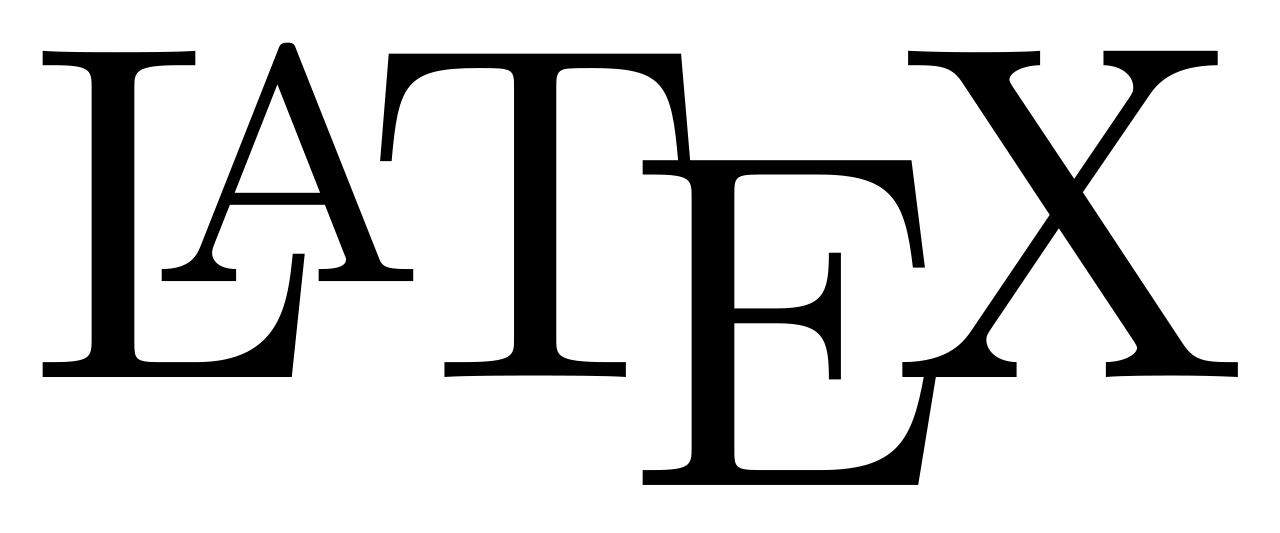
\includegraphics[width=0.5\textwidth]{./logo/LaTex.png}}

\begin{document}
	
	\frame{\titlepage} %标题帧
	
	\begin{frame}\frametitle{Outline}  %设置目录
	\tableofcontents[pausesections]
	\end{frame}
	
	\section{First section}
	\begin{frame}[c]\frametitle{First section}
	The context goes here.   %普通帧
	你好,Beamer!!First section
	\end{frame}

	\section{Second section}
	\begin{frame}[plain]
	这是一个空白帧,没有标题。

	\subsection{First subsection}
	你好,First subsection
	\end{frame}
	
	\section*{Third section}\centering  %带星号不会出现在目录中
	\begin{frame}[c]{Third section}
	你好,Third section.
	\end{frame}

	\begin{frame}[c]\frametitle{无序列表itemize示例}
	\begin{itemize}		%无序列表itemize示例
		\item The first item
		\item The second item
		\item The third item
		\item The fourth item
	\end{itemize}
	\end{frame}

	\begin{frame}[c]{有序列表enumerate示例}
	\begin{enumerate}	%有序列表enumerate示例
		\item The first item
		\item The second item
		\item The third item
		\item The fourth item
	\end{enumerate}
	\end{frame}

	\begin{frame}[c]{描述列表description示例}
	\begin{description}  %描述列表description示例
		\item[First Item] Description of first item
		\item[Second Item] Description of second item
		\item[Third Item] Description of third item
		\item[Forth Item] Description of forth item
	\end{description}
	\end{frame}
	
	\begin{frame}[c]{文本}
	\emph{Sample Text 着重斜体}	\\	  %着重斜体
	\textbf{Sample Text 加粗}	\\	%加粗
	\textit{Sample Text 斜体}	\\	%斜体
	\textsl{Sample Text 用的少的斜体}\\	%用的少的斜体
	\alert{Sample Text 着重警告}\\		%着重警告
	\textrm{Sample Text 正常字体}\\	%正常字体
	\textsf{Sample Text 非衬线字体}\\	%非衬线字体
	\textcolor{green}{Sample Text}\\
	\structure{Sample Text beamer特有的颜色}\\ %beamer特有的structure颜色
	\end{frame}

	\begin{frame}[c]{公式}
	\begin{equation}
	\frac{{- b \pm \sqrt {{b^2} - 4ac} }}{2a}
	\end{equation}
	
	\begin{align}  %align环境每一行都有编号,且可以独立存在,不需要数学环境
	z&=(a+b)^4=(a+b)^2(a+b)^2 \nonumber \\ %以等号作为划分
	&=(a^2+2ab+b^2)(a^2+2ab+b^2)\nonumber \\
	&=a^4+4a^3b+6a^2b^2+4ab^3+b^4		
	\end{align}
	\end{frame}

	\end{document}